\section{Task 1 - Authentication and Registration}
\subsection{The task}
The webapp requires authentication and registration to the server. Authentication should last a defined amount of time.

To do that, at the login page we verify the credentials and then create a new session where we save the username, while for the registration we first create a new set of credentials and then create a similar session.

The credentials are stored in the shared memory of the servlet context. Since it is shared, we need to synchronize the block where we use it. What we save inside it, as the attribute \textit{user} is an array of the class \textit{UserCredentials.java}, which has fields for username and password and is serializable (useful for task 9). It also uses Bean standard, meaning we need to use get and set functions to modify the fields inside (which are private).

Inside the context we also save another attribute \textit{logged}, which contains an array of the class \textit{UserSession.java}. This class contains the fields username and points, which are the same values we save inside the session we give back to the user. It will be useful later for task 8. Like \textit{UserCredentials.java}, it uses Bean standard.
\subsection{Login page}
\subsubsection{login.jsp}
The login jsp page is simple: at the start of the file, we take the \textit{error\_msg} attribute for the request, and if not null we add it in the page in a paragraph.

We also have a form for the login and a link to the Register page.
\subsubsection{Login.java}
For the login page, we have two methods, GET and POST. The GET method simply forwards the request to the \textit{login.jsp} file. For the POST method we loop through each set of credentials that we have: if we cannot find the given username or if the password is not correct, we forward back to the jsp page with an error message. The way we do that is simple: the jsp page accepts an \textit{error\_msg} attribute.

The place where we have saved the credentials of our users is in the context, so at the start of the POST method we use the function \textit{getUsersFromContext} to get all the credentials saved in our system.

If the credentials are ok, we create a new session in the \textit{setSession} function (or we change the current session, if the user went again to the login page), where we save the username and a point filed initialized at zero (as requested in the task 2). This function also modifies the context: it will be explained later, as it is another task objective.


\subsubsection{Screenshots}
\begin{figure}[H]
  \centering
  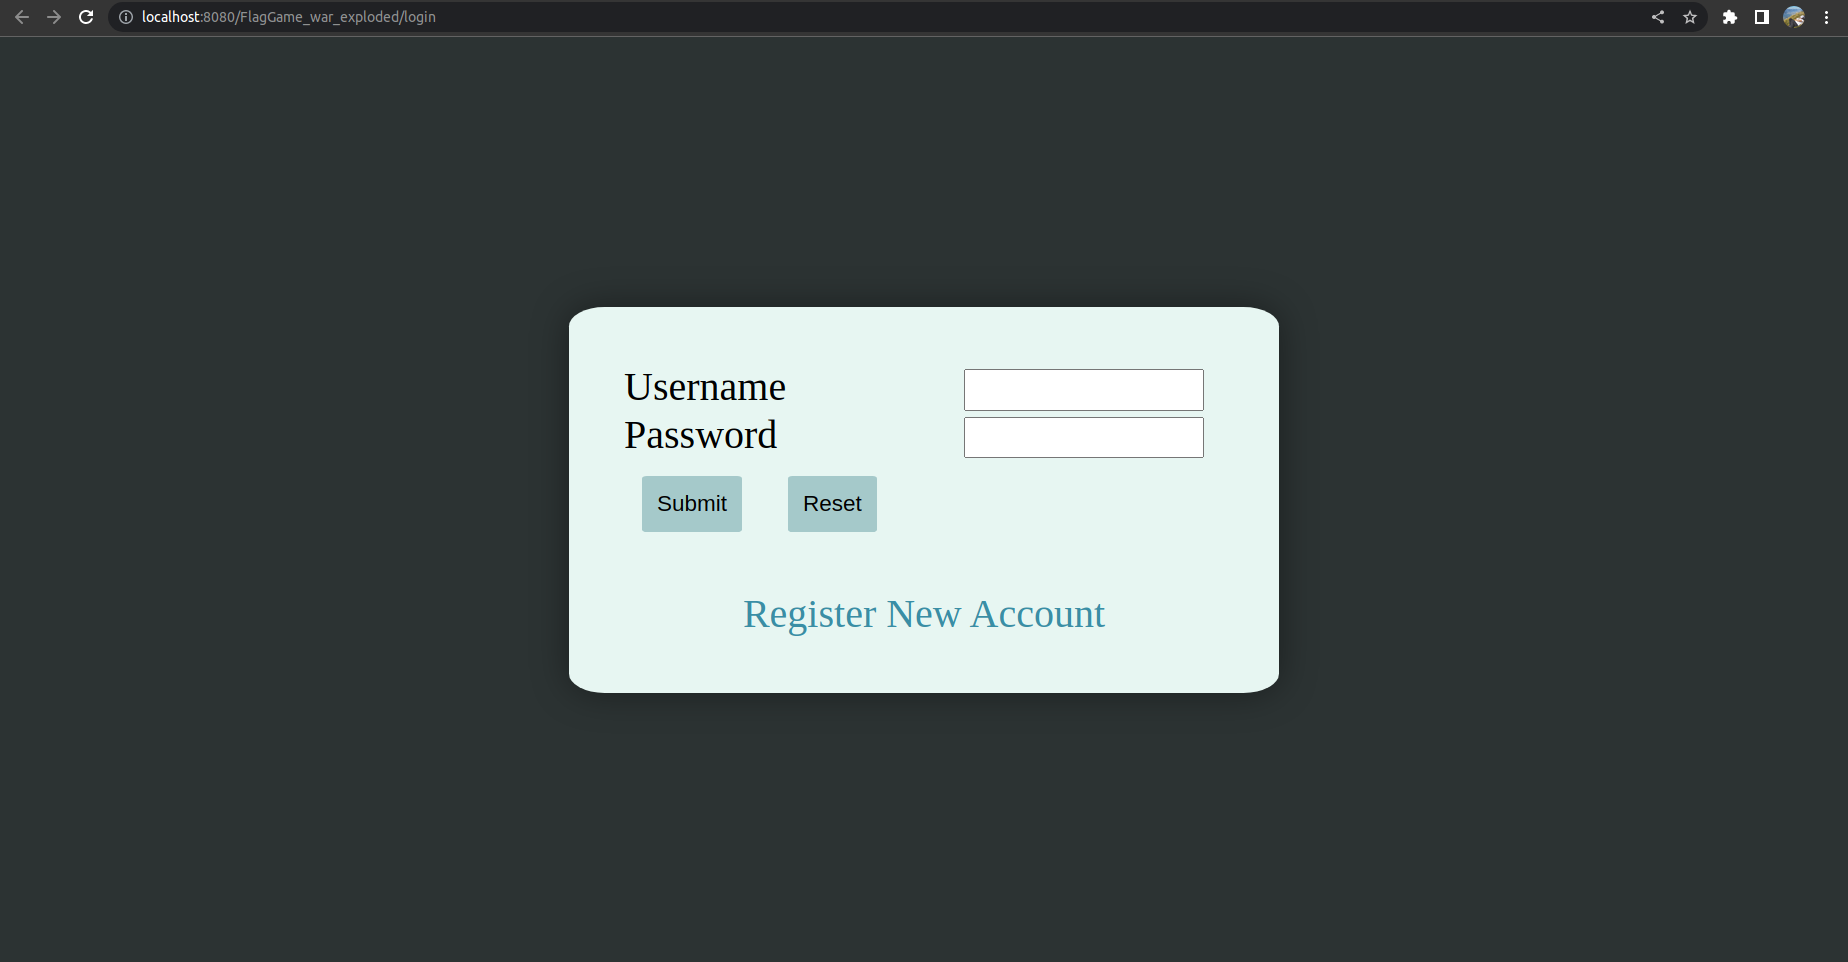
\includegraphics[width=\columnwidth]{login.png}
  \caption{Login Page}
\end{figure}
\begin{figure}[H]
  \centering
  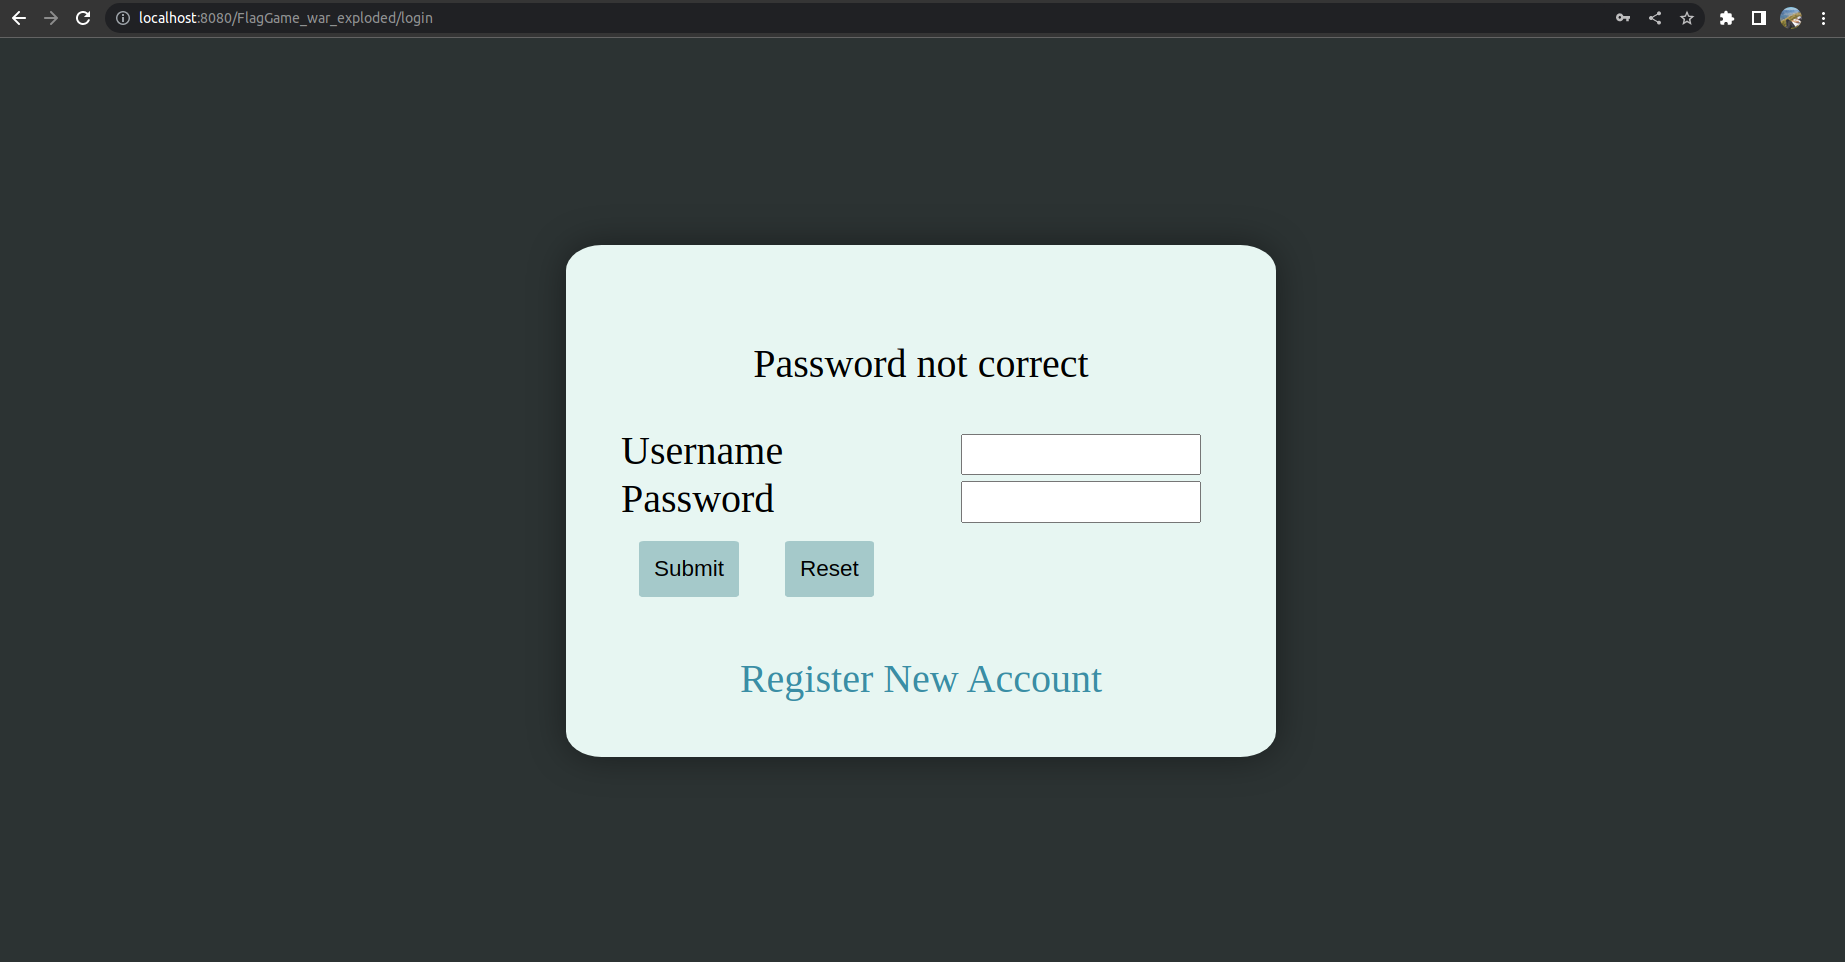
\includegraphics[width=\columnwidth]{login_password_not_correct.png}
  \caption{Login Page if the password is not correct}
\end{figure}
\begin{figure}[H]
  \centering
  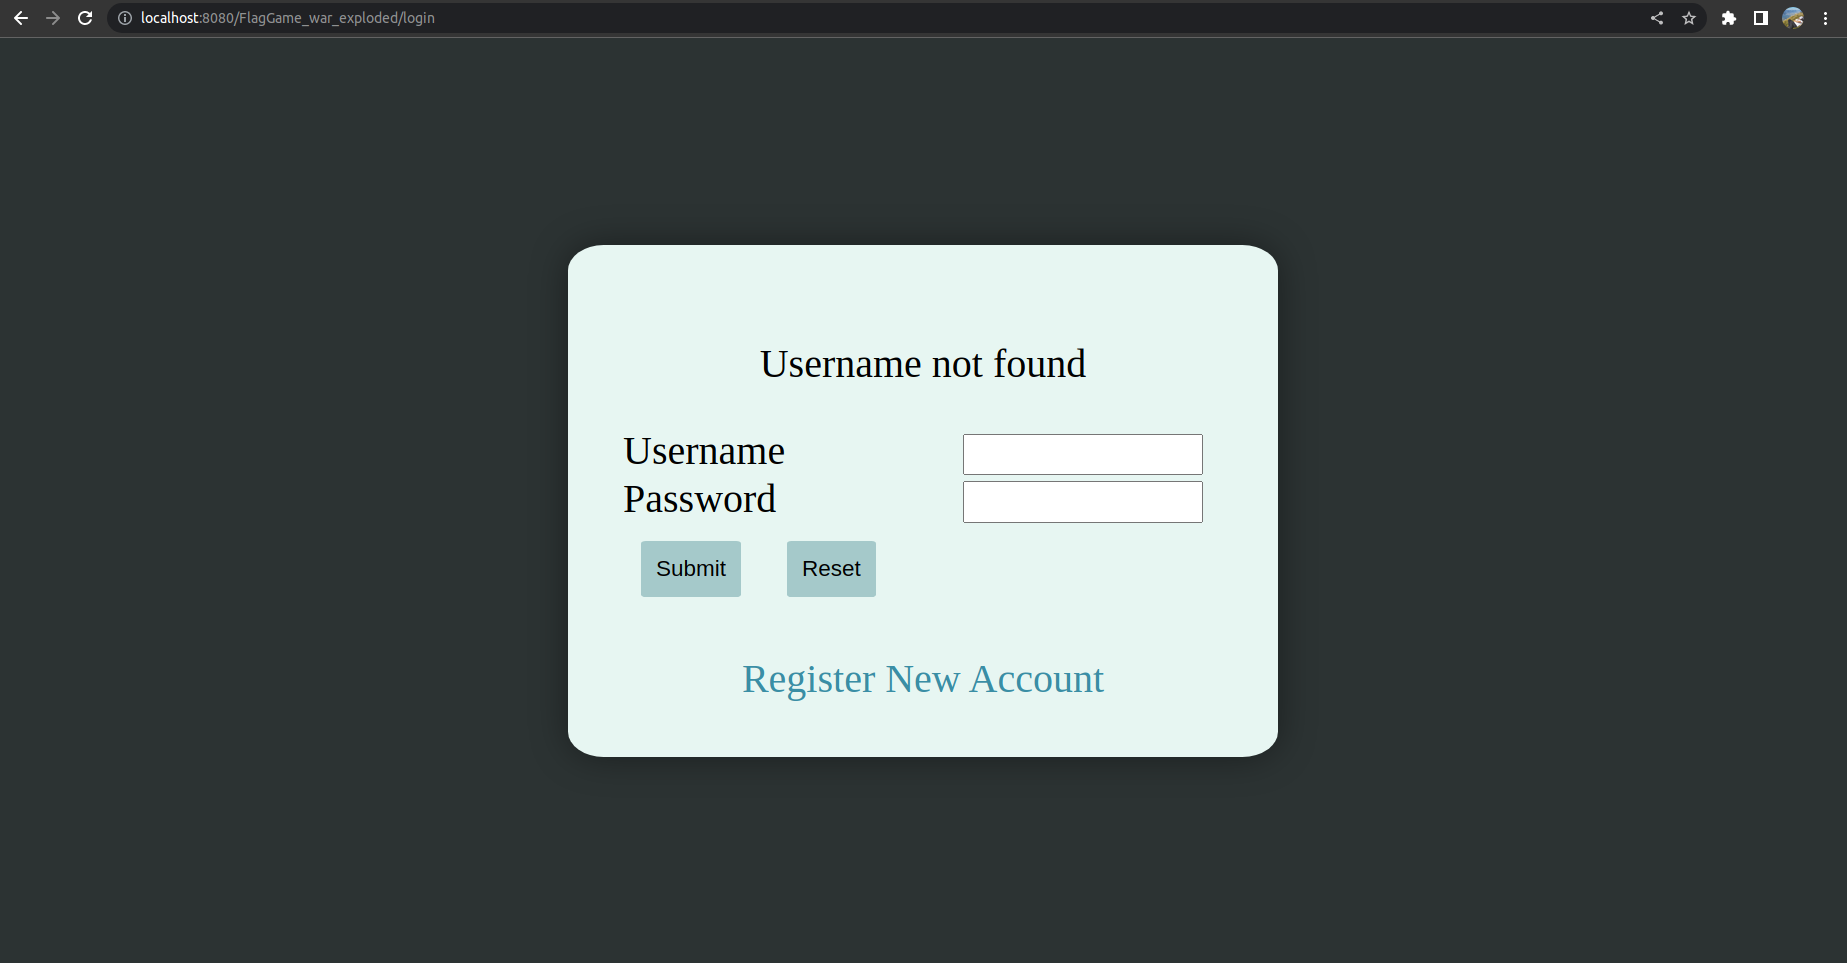
\includegraphics[width=\columnwidth]{login_username_not_found.png}
  \caption{Login Page if the username is not found}
\end{figure}

\subsection{Registration Page}
\subsubsection{register.jsp}
Same logic as \textit{login.jsp}, the only difference is that in the form we have a third field.
\subsubsection{Register.java}
The registration page is very similar: the main difference is that now instead of checking the context for an existing user we add a new one. The checks we do are that the two passwords given are the same and that the username does not already exist.

To get the credentials set and create a new session we use the same functions of \textit{Login.java}, \textit{getUsersFromContext} and \textit{setSession}, so we make these functions static. In particular, at the end of the POST method we modify the context with the new, expanded credentials.


\subsubsection{Screenshots}
\begin{figure}[H]
  \centering
  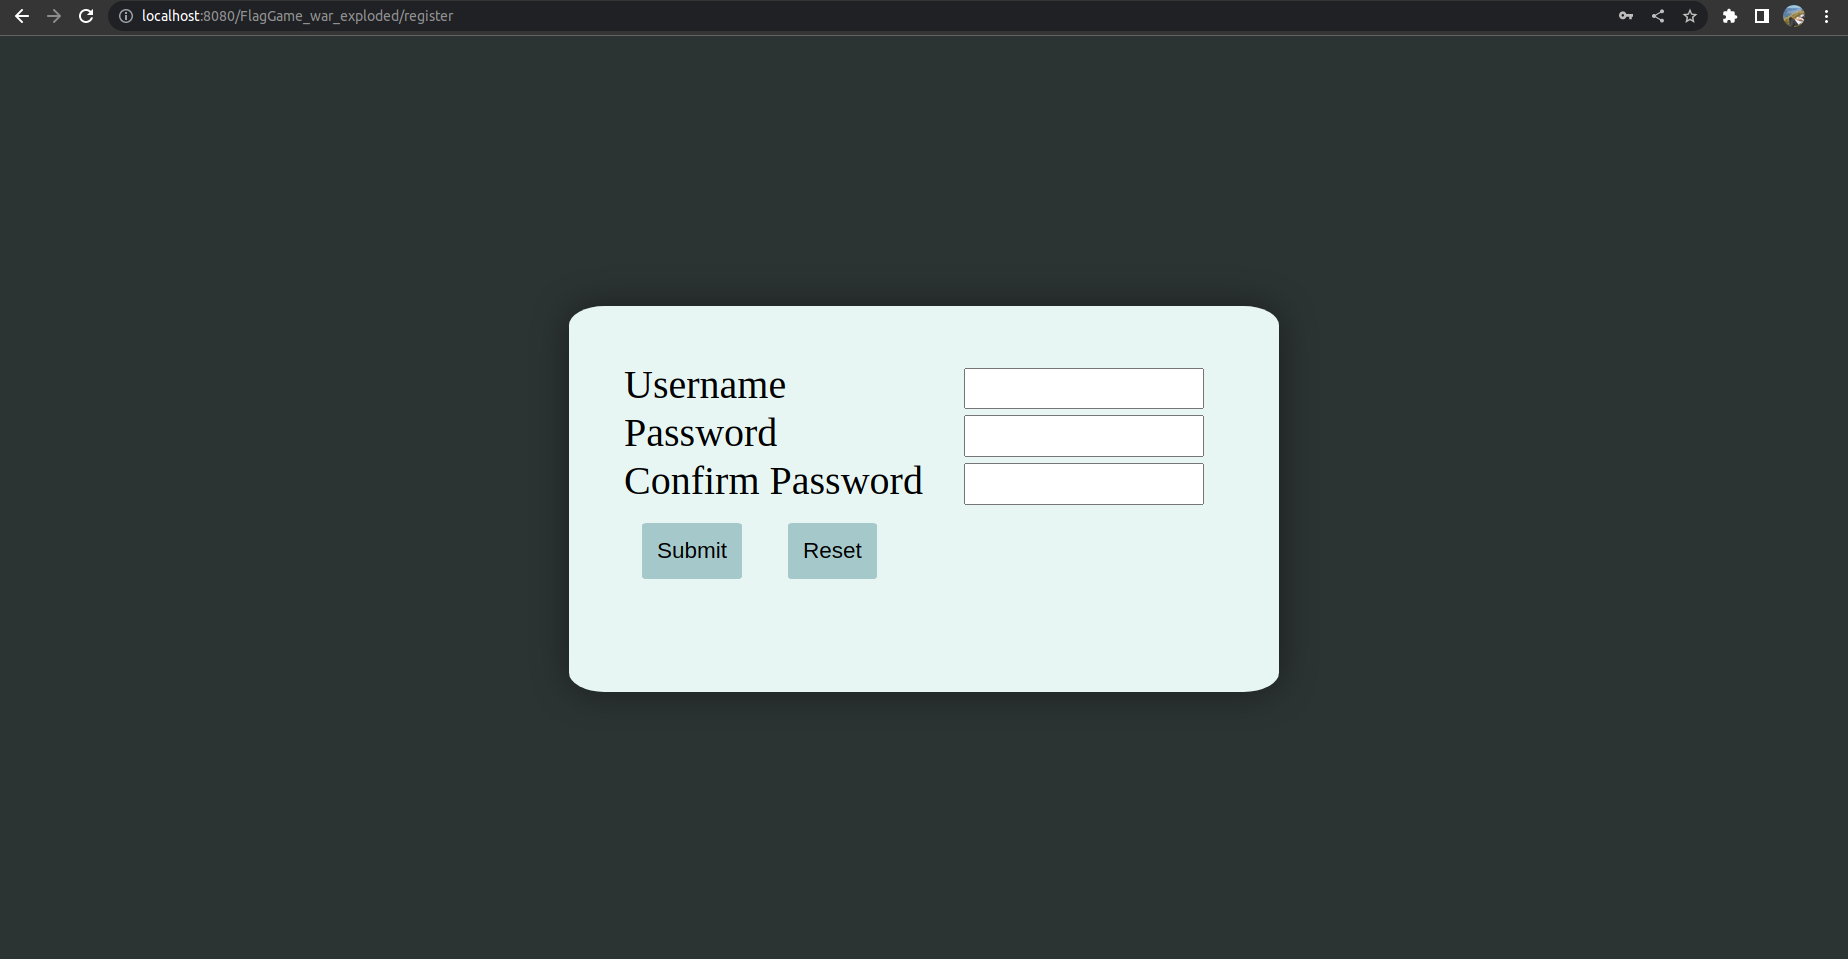
\includegraphics[width=\columnwidth]{register.png}
  \caption{Registration Page}
\end{figure}
\begin{figure}[H]
  \centering
  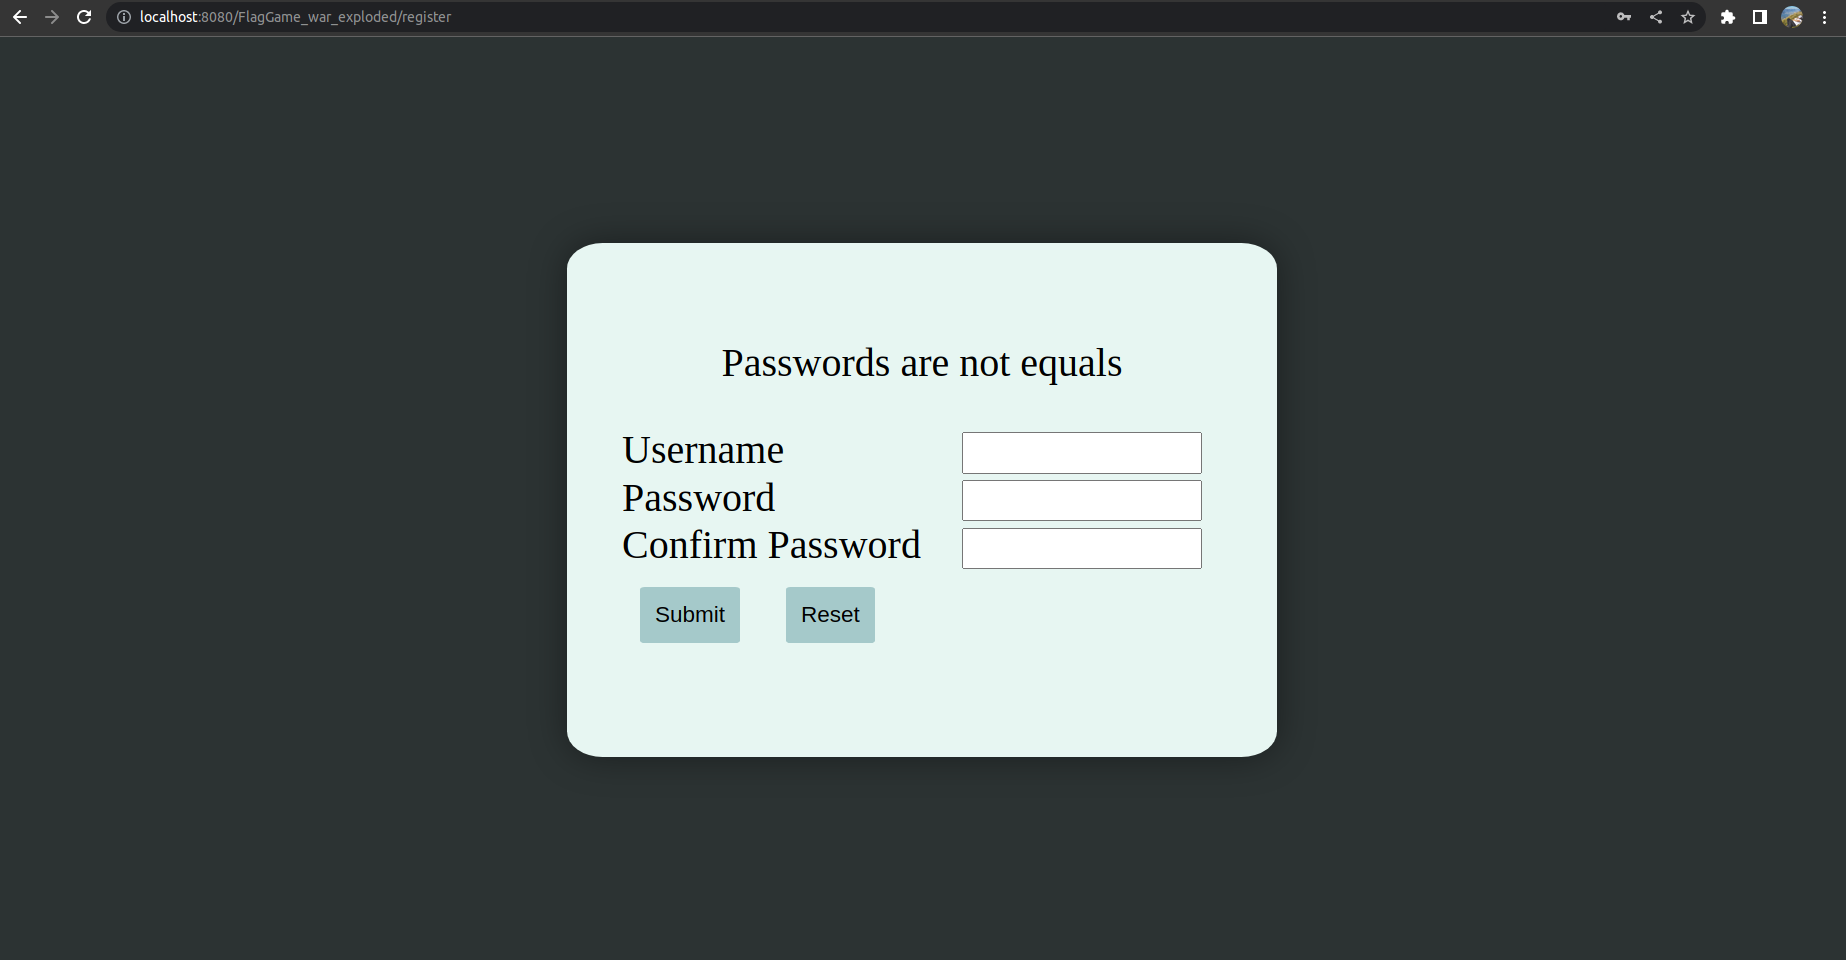
\includegraphics[width=\columnwidth]{register_not_equal_passwords.png}
  \caption{Registration Page if the two passwords given are different}
\end{figure}
\begin{figure}[H]
  \centering
  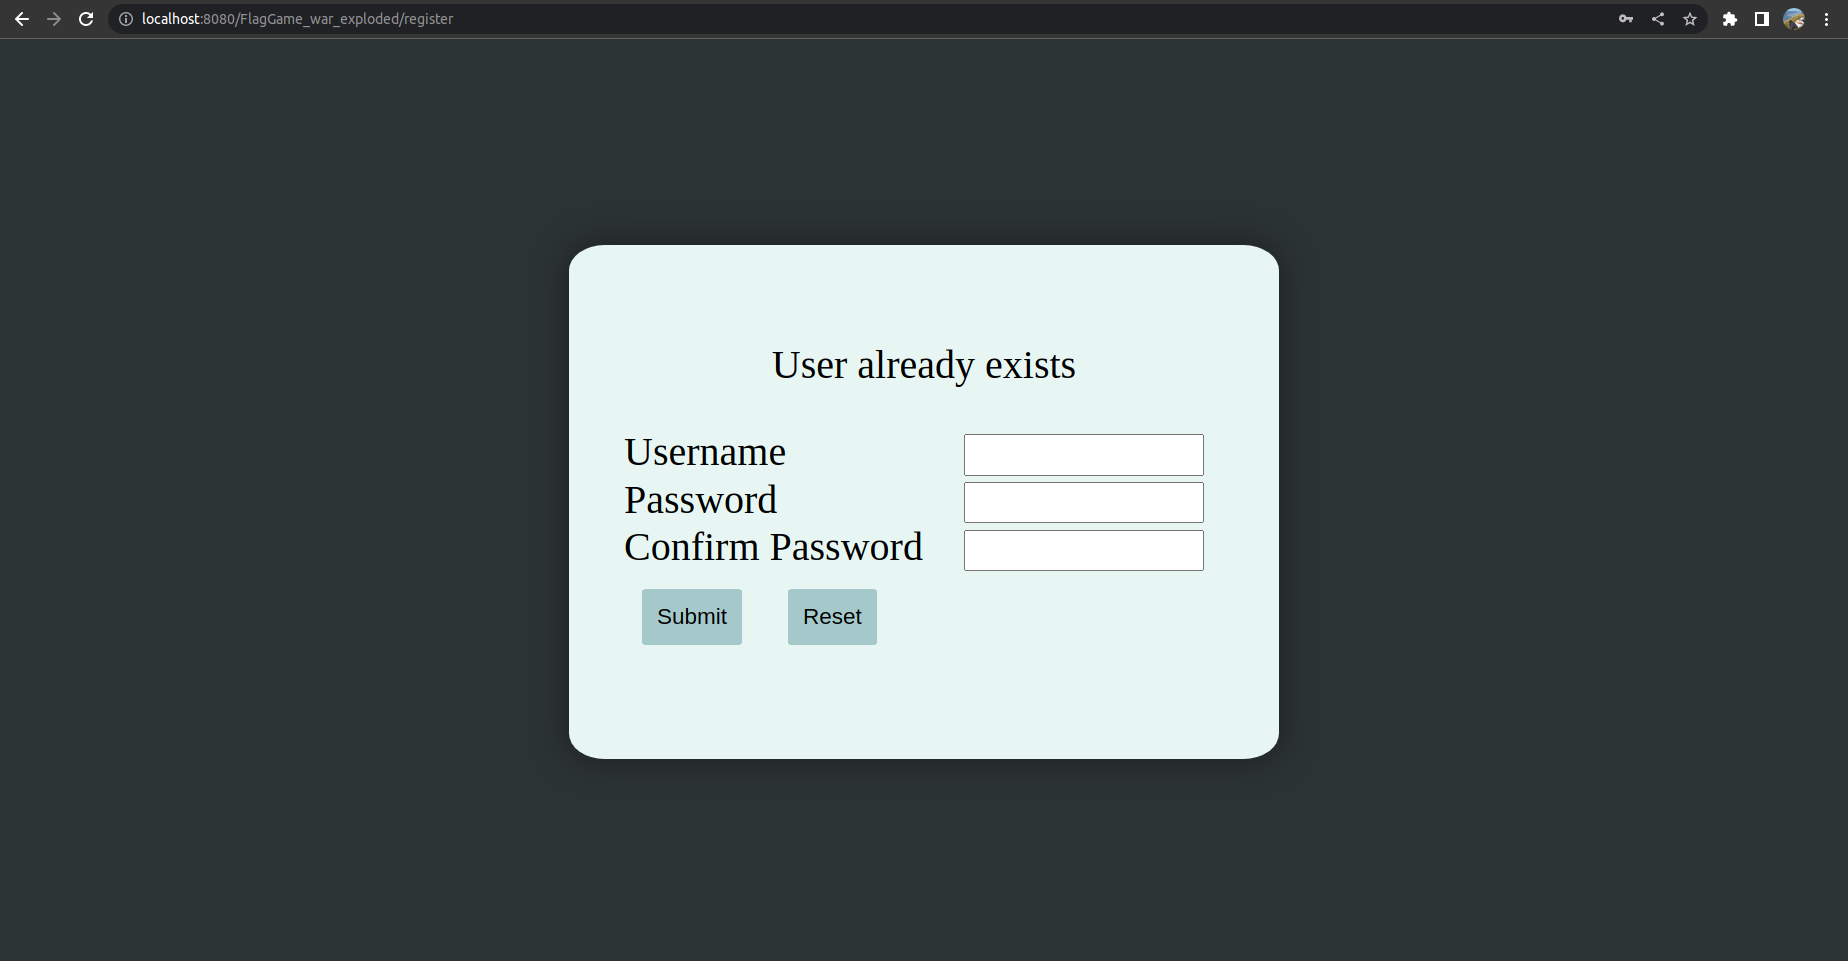
\includegraphics[width=\columnwidth]{register_username_already_exist.png}
  \caption{Registration Page if the username already exists}
\end{figure}